\documentclass[11pt,a4paper]{article}
\usepackage[margin=23mm,headheight=14pt,headsep=8.5mm,footskip=10mm]{geometry}
\usepackage{amsmath,amssymb,amsthm}
\usepackage{assets/tex/cm-bea}
\usepackage{xeCJK}
\setmainfont{Latin Modern Roman}
\setCJKmainfont{FandolSong-Regular.otf}[Script=CustomDefault,Path=assets/fonts/fandol/,BoldFont=FandolSong-Bold.otf,ItalicFont=FandolSong-Regular.otf,BoldItalicFont=FandolSong-Bold.otf]
\setCJKsansfont{FandolSong-Regular.otf}[Script=CustomDefault,Path=assets/fonts/fandol/,BoldFont=FandolSong-Bold.otf]
\xeCJKsetup{PunctStyle=quanjiao,CheckSingle=true}
\usepackage{setspace}
\setstretch{1.12}
\setlength{\parindent}{2em}
\setlength{\parskip}{3pt}
\usepackage{titlesec}
\titleformat{\section}{\centering\normalfont\Large\bfseries}{\thesection.}{0.6em}{}
\titleformat{\subsection}{\normalfont\large\bfseries}{}{0pt}{}
\titlespacing*{\section}{0pt}{1.8\baselineskip}{1.0\baselineskip}
\titlespacing*{\subsection}{0pt}{1.1\baselineskip}{0.5\baselineskip}
\usepackage{enumitem}
\setlist[enumerate]{leftmargin=2em,labelsep=0.5em,itemsep=3pt,parsep=0pt,topsep=6pt}
\providecommand{\tightlist}{\setlength{\itemsep}{3pt}\setlength{\parskip}{0pt}}
\usepackage{needspace}
\newenvironment{statementblock}{\par\Needspace{9\baselineskip}\noindent}{\par\nopagebreak[4]}
\newenvironment{proofblock}{\par\Needspace{4\baselineskip}\noindent}{\par}
\usepackage{fancyhdr}
\pagestyle{fancy}
\fancyhf{}
\fancyhead[L]{\small 数学手记}
\fancyhead[R]{\small 复变函数 · 第七章}
\fancyfoot[C]{\thepage}
\renewcommand{\headrulewidth}{0.4pt}
\usepackage[hidelinks,unicode,bookmarksnumbered=true,linktoc=all]{hyperref}
\usepackage{bookmark}
\bookmarksetup{depth=2}
\hypersetup{pdftitle={复变函数讲义：第七章},pdfauthor={Vincent Arqain},pdfsubject={共形映射}}
\renewcommand{\contentsname}{目录}
\setcounter{tocdepth}{1}
\setcounter{secnumdepth}{1}
\widowpenalty=10000
\clubpenalty=10000
\displaywidowpenalty=10000
\predisplaypenalty=10000
\interdisplaylinepenalty=10000
\raggedbottom

\usepackage{tabularx,booktabs,array}
\renewcommand{\thesection}{7.\arabic{section}}
\emergencystretch=2em

\usepackage{graphicx}
\usepackage{longtable}
\usepackage{calc}
\usepackage{float}
\floatplacement{figure}{H}
\renewcommand{\figurename}{图}
\makeatletter
\def\maxwidth{\ifdim\Gin@nat@width>\linewidth\linewidth\else\Gin@nat@width\fi}
\def\maxheight{\ifdim\Gin@nat@height>0.72\textheight0.72\textheight\else\Gin@nat@height\fi}
\makeatother
\setkeys{Gin}{width=\maxwidth,height=\maxheight,keepaspectratio}
\providecommand{\pandocbounded}[1]{#1}
\setcounter{tocdepth}{2}
\begin{document}
\begin{center}
{\LARGE\bfseries 复变函数讲义\par}
\vspace{8pt}{\large 第七章\quad 共形映射\par}
\vspace{6pt}{\small 依史济怀、刘太顺《复变函数》\quad 教材第 210—234 页\par}
\end{center}\vspace{8pt}
本章含4节讲义及全部 25 道习题原题。定义、定理和性质沿用教材的记号与编号；证明补足必要条件、退化情形与关键推导。覆盖 19 个教材编号条目，补足 Jordan 边界对应、角点展开、无穷远端和积分分支的证明，保留教材配图及提示。§7.1 附七题详解，其余 18 题尚待作答；章末保留全部原题及独立校注。
\begingroup\setlength{\parskip}{0pt}\tableofcontents\endgroup\clearpage
\section{正规族}
对应教材第 210---213 页。记
\(\mathbb D=B(0,1)\)、\(\mathbb H=\{z:\operatorname{Im}z>0\}\)。两个域全纯等价，是指存在从一个域到另一个域的双全纯映射。恒等映射、全纯逆映射和映射复合分别给出自反性、对称性和传递性。本章研究异于
\(\mathbb C\) 的单连通域为何都与 \(\mathbb D\)
等价，以及这种等价怎样延伸到边界。

\subsection*{定理索引}\label{ch07-s1-heading-1}

\hyperref[ch07-s1-heading-2]{定义 7.1.1} · \hyperref[ch07-s1-heading-3]{定义 7.1.2} ·
\hyperref[ch07-s1-heading-4]{定义 7.1.3} · \hyperref[ch07-s1-heading-5]{定理 7.1.4} ·
\hyperref[ch07-s1-heading-6]{定理 7.1.5} · \hyperref[ch07-s1-heading-7]{与下一节的联系}
· \hyperref[ch07-s1-heading-8]{唯一极限判据} · \hyperref[ch07-s1-heading-9]{七题详解}

\Needspace{8\baselineskip}
\subsection{定义 7.1.1：正规族}\label{ch07-s1-heading-2}

域 \(D\) 上的函数族 \(\mathcal F\) 称为正规族，如果其中每个序列都含有在
\(D\) 上内闭一致收敛的子列。``内闭一致''即在每个紧集 \(K\Subset D\)
上一致收敛；本章的极限是有限值函数，不允许恒等于
\(\infty\)，也不要求极限仍属于 \(\mathcal F\)。

全纯函数的此种极限由 Weierstrass 定理仍全纯，各阶导数也内闭一致收敛。族
\(\{z\mapsto n:n\in\mathbb N\}\) 在球面距离意义下可趋于
\(\infty\)，却不是本章意义的正规族：任何子列在任一点的值都无有限极限。不可混用这两种``正规''。

\Needspace{8\baselineskip}
\subsection{定义 7.1.2：一致有界与内闭一致有界}\label{ch07-s1-heading-3}

若存在 \(M\)，使 \(|f(z)|\le M\) 对全部 \(f\in\mathcal F,z\in D\)
成立，称一致有界。若对每个 \(K\Subset D\) 存在 \(M_K\)，使
\(|f(z)|\le M_K\) 对全部 \(f\in\mathcal F,z\in K\)
成立，称内闭一致有界。常数可以依赖 \(K\)，但不能依赖 \(f\)。

一致有界蕴含内闭一致有界，逆命题不成立。例如单元素族 \(\{(1-z)^{-1}\}\)
在 \(\mathbb D\) 的每个紧集上有界，却在 \(z\to1\) 时无界。

\Needspace{8\baselineskip}
\subsection{定义 7.1.3：等度连续}\label{ch07-s1-heading-4}

族 \(\mathcal F\) 在集合 \(E\) 上等度连续，是指对每个
\(\varepsilon>0\)，存在共同的 \(\delta>0\)，使

\[
|z-w|<\delta,\quad z,w\in E
\quad\Longrightarrow\quad |f(z)-f(w)|<\varepsilon\quad(f\in\mathcal F).
\]

逐个函数连续不足以保证这个共同的 \(\delta\)。例如 \(f_n(x)=x^n\) 在
\([0,1]\) 上都连续，但不等度连续：任给 \(\delta>0\)，固定
\(x\in(\max\{0,1-\delta\},1)\)，当 \(n\) 足够大时 \(1-x^n>1/2\)。

\Needspace{8\baselineskip}
\subsection{定理 7.1.4：Arzelà--Ascoli 定理}\label{ch07-s1-heading-5}

设 \(K\subset\mathbb C\) 紧，\(\{f_n\}\) 在 \(K\)
上一致有界且等度连续，则有子列在 \(K\) 上一致收敛。

证明：在 \(K\) 中取可数稠密集 \(A=\{a_j\}_{j\ge1}\)。它可由每级有限的
\(1/m\) 网取并得到。依次在 \(a_1,a_2,\ldots\)
处应用有界复数列的子列收敛性，再取对角子列 \(\{g_k\}\)，便使
\(g_k(a_j)\) 对每个固定 \(j\) 收敛。

给定 \(\varepsilon>0\)，由等度连续选 \(\delta\)，使距离小于 \(\delta\)
时各函数值相差小于 \(\varepsilon/3\)。从 \(A\) 选有限个点
\(a_{j_1},\ldots,a_{j_N}\)，其 \(\delta\) 邻域覆盖 \(K\)。存在
\(k_0\)，当 \(k,l\ge k_0\) 时，这有限多个点上的 \(|g_k-g_l|\) 都小于
\(\varepsilon/3\)。任取 \(z\in K\) 并选 \(|z-a_{j_s}|<\delta\)，则

\[
\begin{aligned}
|g_k(z)-g_l(z)|
&\le |g_k(z)-g_k(a_{j_s})|+|g_k(a_{j_s})-g_l(a_{j_s})|\\
&\quad+|g_l(a_{j_s})-g_l(z)|<\varepsilon.
\end{aligned}\qquad\text{(7.1.1)}
\]

所以 \(\{g_k\}\) 一致 Cauchy。逐点取复数域中的极限，再让
\(l\to\infty\)，即得一致收敛；极限连续。稠密集上的对角法负责``抽出一个候选''，等度连续和有限覆盖负责把逐点控制提升为一致控制。

\Needspace{8\baselineskip}
\subsection{定理 7.1.5：Montel 定理}\label{ch07-s1-heading-6}

全纯函数族 \(\mathcal F\subset H(D)\) 正规，当且仅当它内闭一致有界。

证明：若正规而在某个 \(K\Subset D\) 上不一致有界，可选
\(f_n\in\mathcal F\) 使 \(\sup_K|f_n|>n\)。正规性给出内闭一致收敛子列
\(f_{n_k}\to f\)。连续函数 \(f\) 在 \(K\) 上有界，故充分大的 \(k\) 满足
\(\sup_K|f_{n_k}|\le1+\sup_K|f|\)，与 \(n_k\to\infty\) 矛盾。

反之，设内闭一致有界。给定 \(K\Subset D\)，选 \(r>0\)，使闭 \(3r\) 邻域
\(K_{3r}=\{z:\operatorname{dist}(z,K)\le3r\}\Subset D\)，记共同上界为
\(M\)。对距 \(K\) 不超过 \(r\) 的 \(\zeta\)，圆周 \(|z-\zeta|=r\) 落在
\(K_{3r}\)，Cauchy 估计给出 \(|f'(\zeta)|\le M/r\)。若 \(z,w\in K\) 且
\(|z-w|<r\)，连接它们的线段都在上述邻域，因而

\[
|f(z)-f(w)|\le\frac Mr|z-w|.\qquad\text{(7.1.2)}
\]

这证明在 \(K\)
上等度连续。这里先在较大的紧邻域取上界，再在较小集合估导数，不能把边界附近的导数界从同一个开圆盘的函数界直接省略地推出。

取紧穷竭

\[
K_j=\{z\in D:|z|\le j,\ \operatorname{dist}(z,\mathbb C\setminus D)\ge1/j\}.
\]

若 \(D=\mathbb C\)，改取 \(K_j=\{|z|\le j\}\)。每个 \(K\Subset D\)
最终包含于某个 \(K_j\)。由定理 7.1.4，依次抽出在 \(K_1,K_2,\ldots\)
上一致收敛的嵌套子列，再取对角子列；它在每个 \(K_j\)
上一致收敛，重叠处极限一致，于是定义 \(D\)
上的极限函数并内闭一致收敛。由 Weierstrass 定理极限全纯。

\subsection*{与下一节的联系：极值为什么可以达到}\label{ch07-s1-heading-7}

对 \(\mathbb D\) 值全纯函数，Montel 自动给出收敛子列，但极限起初只能满足
\(|f|\le1\)；用最大模原理，只有排除常值退化后才可断言
\(|f|<1\)。单叶函数列的内闭一致极限也可能退化为常数，例如
\(f_n(z)=z/n\)。下一节固定 \(f(a)=0\)，并使 \(f'(a)\)
趋于一个正上确界，正是用导数防止这两种退化。

\subsection*{补充性质：唯一子列极限与整列收敛}\label{ch07-s1-heading-8}

设 \(\{f_n\}\subset H(D)\)
内闭一致有界。若它的所有内闭一致收敛子列都有同一个极限
\(f\)，则整列内闭一致收敛于 \(f\)。

证明：Montel 定理先保证至少有一个这样的子列，故
\(f\in H(D)\)。若整列不内闭一致收敛于 \(f\)，则存在
\(K\Subset D\)、\(\varepsilon_0>0\) 及子列 \(\{f_{n_k}\}\)，使

\[
\sup_{z\in K}|f_{n_k}(z)-f(z)|\ge\varepsilon_0\qquad(k\ge1).
\qquad\text{(7.1.3)}
\]

再对这个子列应用 Montel 定理，可取内闭一致收敛的子子列；其极限按假设仍为
\(f\)，与式 (7.1.3)
矛盾。这一性质把``能抽取收敛子列''和``所有候选极限相同''合成整列收敛，以下前三题及第七题都使用它。

\subsection*{习题 7.1 详解}\label{ch07-s1-heading-9}

题目对应教材印刷第 213
页，保留原题编号与全部条件。\hyperref[ch07-practice-heading-2]{独立原题页}继续用于练习；本节给出七题的完整解答。

\hyperref[ch07-s1-ux95eeux9898-711]{问题 7.1.1} ·
\hyperref[ch07-s1-ux95eeux9898-712]{问题 7.1.2} ·
\hyperref[ch07-s1-ux95eeux9898-713]{问题 7.1.3} ·
\hyperref[ch07-s1-ux95eeux9898-714]{问题 7.1.4} ·
\hyperref[ch07-s1-ux95eeux9898-715]{问题 7.1.5} ·
\hyperref[ch07-s1-ux95eeux9898-716]{问题 7.1.6} ·
\hyperref[ch07-s1-ux95eeux9898-717]{问题 7.1.7}

\subsubsection{问题 7.1.1}\label{ch07-s1-ux95eeux9898-711}

设 \(\{f_n\}\) 是域 \(D\) 上的全纯函数列，并且在 \(D\)
上内闭一致有界。证明：若 \(\lim_{n\to\infty}f_n(z)\) 在 \(D\)
上处处存在，则 \(\{f_n\}\) 在 \(D\) 上内闭一致收敛。

证明：记逐点极限为 \(F\)。Montel 定理给出内闭一致收敛子列
\(f_{n_k}\to f\in H(D)\)。对每个 \(z\in D\)，同一子列又逐点收敛于
\(F(z)\)，所以 \(f=F\)。任意其他内闭一致收敛子列也只能以 \(F\)
为极限，由唯一子列极限性质，整列内闭一致收敛于
\(F\)。这里同时证明了逐点极限的全纯性，没有预先假定 \(F\) 连续或全纯。

\subsubsection{问题 7.1.2}\label{ch07-s1-ux95eeux9898-712}

设 \(\{f_n\}\) 是域 \(D\) 上的全纯函数列，并且在 \(D\)
上内闭一致有界，\(A=\{z=x+iy\in D:x,y\text{ 为有理数}\}\)。证明：若
\(\lim_{n\to\infty}f_n(z)\) 在 \(A\) 上处处存在，则 \(\{f_n\}\) 在 \(D\)
上内闭一致收敛。

证明：开集 \(D\)
的每个点附近都含一个小圆盘，其中可选实部、虚部均为有理数的点，故 \(A\)
在 \(D\) 中稠密。由 Montel 定理至少有一个内闭一致子列极限。若 \(f,g\)
是任意两个这样的极限，则对每个 \(a\in A\)，二者都等于已存在的
\(\lim_n f_n(a)\)，所以 \(f=g\) 于 \(A\)。它们连续，由稠密性知 \(f=g\)
于 \(D\)。唯一子列极限性质遂给出整列内闭一致收敛。

此题靠稠密性与连续性识别极限；下一题的点集不必稠密，须改用全纯函数的唯一性定理。

\subsubsection{问题 7.1.3}\label{ch07-s1-ux95eeux9898-713}

（Vitali 定理）设 \(\{f_n\}\) 是域 \(D\) 上的全纯函数列，并且在 \(D\)
上内闭一致有界，\(\{z_j\}\) 是 \(D\)
中彼此不同的点列，\(z_j\to z_0\in D\)。证明：若
\(\lim_{n\to\infty}f_n(z)\) 在 \(\{z_j\}\) 上处处存在，则 \(\{f_n\}\) 在
\(D\) 上内闭一致收敛。

证明：由 Montel 定理，内闭一致收敛子列存在，所有这种极限都是 \(D\)
上全纯函数。若 \(f,g\) 为其中任意两个，则对每个固定的 \(j\)，

\[
f(z_j)=\lim_{n\to\infty}f_n(z_j)=g(z_j).
\qquad\text{(7.1.4)}
\]

因为 \(z_j\) 互异且聚于域内的 \(z_0\)，唯一性定理给出 \(f\equiv g\)
于连通域
\(D\)。再由唯一子列极限性质，整列内闭一致收敛。将原题的点列下标改记为
\(j\)，只是为了明确式 (7.1.4)
对每个固定点取函数列的极限；题设不是仅要求对角值 \(f_n(z_n)\) 收敛。

例如 \(f_n(z)=(-1)^n z\) 在 \(\mathbb D\) 上一致有界，对互异点
\(z_n=1/(n+1)\) 有
\(f_n(z_n)\to0\)，但整列在任意固定的非零点都不收敛。这说明仅有对角值收敛不足以应用本题。

\subsubsection{问题 7.1.4}\label{ch07-s1-ux95eeux9898-714}

设 \(\mathcal F\) 是域 \(D\)
上的全纯函数族，\(z_0\in D\)。证明：若（1）\(\operatorname{Re}f(z)\ge0\)
对所有 \(z\in D\)、\(f\in\mathcal F\) 成立；（2）\(f(z_0)=g(z_0)\)
对所有 \(f,g\in\mathcal F\) 成立，则 \(\mathcal F\)
正规。并举例说明条件（2）不可去掉。

证明：空族的结论显然，以下设公共值为 \(a=\alpha+i\beta\)，其中
\(\alpha\ge0\)。若 \(\alpha=0\)，则对任意 \(f\in\mathcal F\)，全纯函数
\(e^{-f}\) 满足 \(|e^{-f}|\le1\) 且在 \(z_0\) 取模 \(1\)。最大模原理给出
\(e^{-f}\) 为常数，求导得 \(f'\equiv0\)，故 \(f\equiv i\beta\)。这时
\(\mathcal F\) 至多含一个函数，当然正规。

若 \(\alpha>0\)，令

\[
h_f(z)=\frac{f(z)-a}{f(z)+\overline a}.
\qquad\text{(7.1.5)}
\]

分母的实部至少为 \(\alpha\)，所以 \(h_f\) 全纯；并且

\[
\begin{aligned}
|f(z)+\overline a|^2-|f(z)-a|^2
&=4\alpha\operatorname{Re}f(z)\ge0,\\
|h_f(z)|&\le1,\qquad h_f(z_0)=0.
\end{aligned}
\qquad\text{(7.1.6)}
\]

任取序列 \(\{f_n\}\subset\mathcal F\)，对有界族 \(\{h_{f_n}\}\) 应用
Montel 定理，可取子列 \(h_{f_{n_k}}\to h\)
内闭一致。极限全纯，\(|h|\le1\) 且 \(h(z_0)=0\)，最大模原理遂给出
\(|h(z)|<1\) 于 \(D\)。由式 (7.1.5) 解得

\[
f_{n_k}=\frac{a+\overline a h_{f_{n_k}}}{1-h_{f_{n_k}}}
\longrightarrow F=\frac{a+\overline a h}{1-h}.
\qquad\text{(7.1.7)}
\]

此收敛在每个紧集 \(K\Subset D\) 上一致：先取
\(q=\max_K|h|<1\)，再由一致收敛使充分大的 \(k\) 满足
\(\max_K|h_{f_{n_k}}|\le(1+q)/2<1\)，从而式 (7.1.7)
的两分母均有共同正下界，分子一致收敛。因此任意序列都有有限值内闭一致收敛子列，\(\mathcal F\)
正规。

若去掉（2），常值族 \(f_n(z)=n\)
的实部均非负，但任意子列在任一点都趋于无穷，故不是本章有限值意义下的正规族。

\subsubsection{问题 7.1.5}\label{ch07-s1-ux95eeux9898-715}

设 \(\mathcal F\) 是域 \(D\) 上的正规全纯函数族，\(g\)
是整函数。证明：\(\{g\circ f:f\in\mathcal F\}\) 也是 \(D\) 上的正规族。

证明：任取复合函数序列 \(g\circ f_n\)，其中
\(f_n\in\mathcal F\)。正规性给出子列 \(f_{n_k}\to f\) 内闭一致，且
\(f\in H(D)\)。固定 \(K\Subset D\)，一致收敛使 \(f_{n_k}(K)\) 与
\(f(K)\) 在充分大的 \(k\) 时都包含于某个闭圆盘
\(\overline{B(0,R)}\)。整函数 \(g\) 在此闭圆盘上一致连续，故
\(g\circ f_{n_k}\to g\circ f\) 在 \(K\) 上一致。因为 \(K\)
任意，得到所需的内闭一致收敛子列。不能仅凭 \(g\)
逐点连续就省去紧集像上的一致控制。

\subsubsection{问题 7.1.6}\label{ch07-s1-ux95eeux9898-716}

设 \(D\) 是有界域，\(0<M<\infty\)。证明函数族

\[
\mathcal F=\left\{f\in H(D):\iint_D|f(z)|^2\,dx\,dy\le M\right\}
\]

在 \(D\) 上正规。

证明：固定非空紧集 \(K\Subset D\)，取 \(r>0\)，使每个 \(z\in K\)
的闭圆盘 \(\overline{B(z,r)}\) 都包含于 \(D\)。由 Cauchy 平均值公式及
Cauchy--Schwarz 不等式，对 \(0<t\le r\) 有

\[
\begin{aligned}
f(z)&=\frac1{2\pi}\int_0^{2\pi}f(z+te^{i\theta})\,d\theta,\\
|f(z)|^2&\le\frac1{2\pi}\int_0^{2\pi}|f(z+te^{i\theta})|^2\,d\theta.
\end{aligned}
\qquad\text{(7.1.8)}
\]

将第二式乘以 \(2\pi t\) 后从 \(0\) 积到 \(r\)，由极坐标换元得到

\[
\begin{aligned}
\pi r^2|f(z)|^2
&\le\int_0^r\int_0^{2\pi}|f(z+te^{i\theta})|^2t\,d\theta\,dt\\
&=\iint_{B(z,r)}|f(\zeta)|^2\,dA(\zeta)\le M.
\end{aligned}
\qquad\text{(7.1.9)}
\]

因此 \(\sup_K|f|\le\sqrt{M/\pi}/r\)，右端与 \(f\) 无关。\(\mathcal F\)
内闭一致有界，由 Montel 定理正规。证明只用已知的 Cauchy
公式，不借用第八章次调和理论；事实上，有界域假设可去掉，只要同一个全域平方积分上界仍成立。

\subsubsection{问题 7.1.7}\label{ch07-s1-ux95eeux9898-717}

设 \(\{f_n\}\) 是域 \(D\) 上的全纯函数列，并且内闭一致有界。证明：若存在
\(z_0\in D\)，使 \(f_n(z_0)\to A\)，且每个 \(f_n\) 都不取值 \(A\)，则
\(f_n\) 在 \(D\) 上内闭一致收敛于常数 \(A\)。

证明：Montel 定理保证内闭一致收敛子列存在。设任一这样的子列
\(f_{n_k}\to f\in H(D)\)，则 \(f(z_0)=A\)。若 \(f-A\)
不恒为零，可取充分小的 \(r>0\)，使 \(\overline{B(z_0,r)}\subset D\)，且
\(f-A\) 在该闭圆盘中仅在中心有零点。令
\(m=\min_{|z-z_0|=r}|f(z)-A|>0\)。充分大的 \(k\) 满足

\[
|f_{n_k}(z)-f(z)|<m\le|f(z)-A|
\quad(|z-z_0|=r).
\qquad\text{(7.1.10)}
\]

Rouché 定理表明 \(f_{n_k}-A\) 与 \(f-A\)
在圆盘内零点个数相同，按重数计至少为一，这与每个 \(f_n\) 都不取值 \(A\)
矛盾。因此 \(f\equiv A\)。所有内闭一致子列极限都只能是常数
\(A\)，唯一子列极限性质给出整列内闭一致收敛于
\(A\)。这也具体展开了本题所用的 Hurwitz 无零点极限结论。

七题的共同方法是先取得紧性，再识别极限。第 1---3
题逐次减弱给定取值的点集，第 4 题用固定点值排除 Cayley 逆变换的退化，第
5 题在紧集像上处理复合，第 6 题由积分控制推出局部上界，第 7
题用零点稳定性强制极限为常数。

\section{Riemann 映射定理}
对应教材第 214---218
页。正规族提供收敛子列；本节把``存在共形映射''转化为归一化单叶函数族中的导数极大问题。全纯对数和平方根使用第六章单值性定理；导数收敛与单叶极限使用第四章的结论。

\subsection*{定理索引}\label{ch07-s2-heading-1}

\hyperref[ch07-s2-heading-2]{定理 7.2.1} · \hyperref[ch07-s2-heading-3]{定理 7.2.2} ·
\hyperref[ch07-s2-heading-4]{正规化、映射半径与条件校注}

\Needspace{8\baselineskip}
\subsection{定理 7.2.1：Riemann 映射定理}\label{ch07-s2-heading-2}

设 \(G\subsetneq\mathbb C\) 是单连通域，\(a\in G\)。存在唯一双全纯映射
\(f:G\to\mathbb D\)，满足

\[
f(a)=0,\qquad f'(a)>0.\qquad\text{(7.2.1)}
\]

这里``\(>0\)''表示导数为正实数，同时固定了尺度的方向。

证明：取 \(b\notin G\)。由单连通性，\(z-b\) 有全纯平方根 \(g\)。若
\(g(z_1)=g(z_2)\)，平方后得 \(z_1=z_2\)，所以 \(g\) 单叶；并且
\(g(G)\cap[-g(G)]=\varnothing\)，否则平方后会迫使同一点的根同时等于两个相反非零值。取
\(\delta>0\) 使 \(B(g(a),\delta)\subset g(G)\)，便有
\(B(-g(a),\delta)\cap g(G)=\varnothing\)，故

\[
\psi(z)=\frac1{g(z)+g(a)},\qquad |\psi(z)|\le\delta^{-1}.
\qquad\text{(7.2.2)}
\]

\(\psi\) 仍单叶。将 \(\psi(z)-\psi(a)\)
乘以充分小的正数和适当单位复数，得到 \(F_0:G\to\mathbb D\)，满足
\(F_0(a)=0,F_0'(a)>0\)。这个构造使任意真单连通域都有一个有界的单叶坐标，不必假设
\(G\) 原来有界。

定义

\[
\mathcal F=\{F:G\to\mathbb D:\ F\text{ 全纯单叶},\ F(a)=0,\ F'(a)>0\}.
\]

已知 \(F_0\in\mathcal F\)。取 \(\overline{B(a,r)}\subset G\)，Cauchy
估计给出 \(F'(a)\le1/r\)，所以

\[
0<M=\sup_{F\in\mathcal F}F'(a)<\infty.
\]

选 \(F_n'(a)\to M\)。Montel 定理给出子列内闭一致收敛于 \(F_*\)，且
\(F_*(a)=0,F_*'(a)=M>0\)，故 \(F_*\) 非常数。最大模原理将 \(|F_*|\le1\)
改进为 \(|F_*|<1\)。为明确单叶性，固定 \(p\in G\)，函数

\[
Q_n(z)=\begin{cases}\dfrac{F_n(z)-F_n(p)}{z-p},&z\ne p,\\F_n'(p),&z=p\end{cases}
\]

在 \(G\) 全纯且无零点，内闭一致趋于相应的 \(Q\)。Hurwitz 定理说明 \(Q\)
恒零或处处非零；恒零将使 \(F_*\) 为常数，已经排除。因此 \(F_*\)
单叶且属于 \(\mathcal F\)，达到导数上确界。

若 \(F_*(G)\ne\mathbb D\)，取遗漏值
\(u\in\mathbb D\setminus F_*(G)\)，则 \(0<\rho=|u|<1\)。令

\[
T_u(w)=\frac{u-w}{1-\bar u w},\qquad v=T_u\circ F_*.
\]

\(v\) 无零点，在单连通的 \(G\) 上取全纯根 \(s^2=v\)。它单叶，且
\(|s|<1\)。记 \(s_0=s(a)\)，则 \(s_0^2=u,|s_0|=\sqrt\rho\)。再令

\[
W(z)=\frac{s_0}{|s_0|}\frac{s_0-s(z)}{1-\bar s_0s(z)}.
\qquad\text{(7.2.3)}
\]

这是 \(G\) 到 \(\mathbb D\) 的单叶全纯映射，且
\(W(a)=0\)。直接用链式法则，注意 \(T_u'(0)=-(1-|u|^2)\)，得到

\[
\begin{aligned}
W'(a)&=\frac{1-\rho^2}{2|s_0|(1-|s_0|^2)}M\\
&=\frac{1+\rho}{2\sqrt\rho}M>M,
\end{aligned}\qquad\text{(7.2.4)}
\]

因为 \((1-\sqrt\rho)^2>0\)。于是 \(W\in\mathcal F\)
却超过上确界，矛盾。故 \(F_*(G)=\mathbb D\)。

\noindent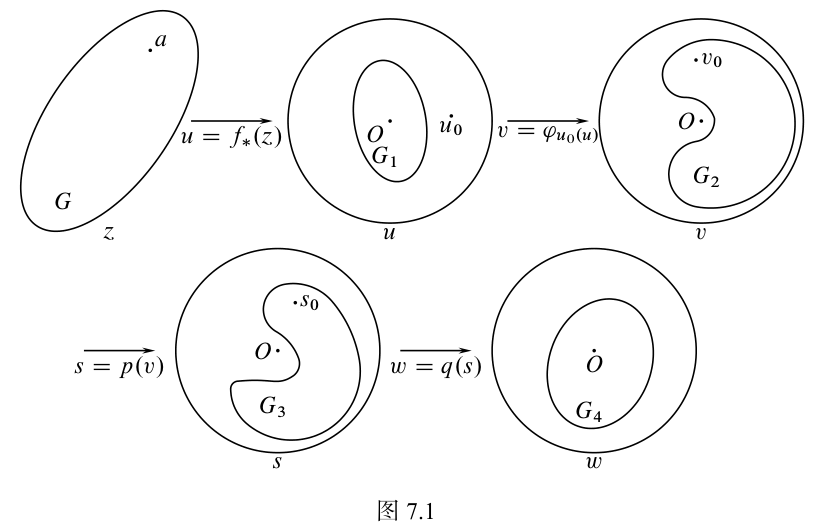
\includegraphics{public/figures/complex-functions/ch07-fig-7-1.png}

若 \(f,g\) 都满足要求，\(f\circ g^{-1}\) 是固定 \(0\)
的圆盘自同构。对它及其逆应用 Schwarz 引理，得到
\(f\circ g^{-1}(z)=e^{i\theta}z\)。其在 \(0\) 的导数
\(f'(a)/g'(a)>0\)，所以 \(e^{i\theta}=1\)，即 \(f=g\)。

平方根构造的动机是：若极值映射还遗漏一点，就先把遗漏点移到原点，使平方根存在；开平方后再把基点移回原点，导数恰增大
\((1+\rho)/(2\sqrt\rho)\)
倍。只说``极值映射应当满射''并不能代替这个计算。

\Needspace{8\baselineskip}
\subsection{定理 7.2.2：两个真单连通域的归一化等价}\label{ch07-s2-heading-3}

设 \(G,D\subsetneq\mathbb C\)
单连通，\(z_0\in G,w_0\in D\)。存在唯一双全纯映射 \(f:G\to D\)，满足
\(f(z_0)=w_0,f'(z_0)>0\)。

证明：取定理 7.2.1 给出的归一化映射
\(g:G\to\mathbb D\)、\(h:D\to\mathbb D\)，分别将 \(z_0,w_0\) 映为
\(0\)。则 \(f=h^{-1}\circ g\) 满足条件，且
\(f'(z_0)=g'(z_0)/h'(w_0)>0\)。若有另一映射 \(F\)，则
\(h\circ F\circ g^{-1}\) 固定 \(0\) 且导数为正，是恒等映射，故 \(F=f\)。

全平面不与 \(\mathbb D\) 全纯等价，因为从 \(\mathbb C\) 到 \(\mathbb D\)
的全纯函数由 Liouville
定理必为常数。因此平面单连通域恰有两个全纯等价类。双全纯映射是同胚，故保持单连通性：闭路及其收缩同伦可用映射和逆映射搬运。对于多连通域，拓扑类型相同还不够；第六章的圆环模数说明
\(r<|z|<R\) 的全纯等价类仍依赖 \(R/r\)。

\subsection*{正规化、映射半径与条件校注}\label{ch07-s2-heading-4}

将 \(f:G\to\mathbb D\) 按定理归一化，\(R_G(a)=1/f'(a)\)
称为映射半径。这是 \(\mathbb D\to G\) 的逆映射在 \(0\)
的正导数。若仅指定 \(f(a)=0\) 而不固定导数方向，仍允许任意旋转
\(e^{i\theta}f\)；若指定三个有序边界点，则必须先证明下一节的边界延拓，不能提前使用。

教材第 215 页极限论证中``\(f_*'\) 不是常数''应为``\(f_*\)
不是常数''：需要的是 \(f_*'(a)=M>0\)，导函数完全可以为正常数。图 7.1
后记号应始终保持 \(v_0=T_u(0)=u\)，不能在同一计算中改成
\(-u\)。以上均在本节用统一记号重算。

\section{边界对应定理}
对应教材第 218---222 页。Riemann 映射只控制域内。边界是 Jordan
曲线时，结论可加强为闭域同胚；如果边界带有裂缝，同一几何点可能有不同的到达侧，不能直接断言边界一一对应。

\subsection*{定理索引}\label{ch07-s3-heading-1}

\hyperref[ch07-s3-heading-2]{定理 7.3.1} · \hyperref[ch07-s3-heading-3]{定理 7.3.2} ·
\hyperref[ch07-s3-heading-4]{例 7.3.3} ·
\hyperref[ch07-s3-heading-5]{边界条件的适用范围}

\Needspace{8\baselineskip}
\subsection{定理 7.3.1：Jordan 域的边界对应定理}\label{ch07-s3-heading-2}

设 \(G\) 为简单闭曲线 \(\Gamma\) 的有界内部，\(f:G\to\mathbb D\)
双全纯。则 \(f\) 唯一地连续延拓为 \(\overline G\to\overline{\mathbb D}\)
的同胚，且保持边界正向。此处不要求 \(\Gamma\) 光滑或可求长。

证明：记 \(\phi=f^{-1}\)，先证明 \(\phi\) 连续到圆周。以下只使用 Jordan
曲线分割定理及其横截弧结论，不预先假定边界映射存在。

\textbf{小横截弧的拓扑事实。} 固定 \(w_0\in G\)。若简单弧 \(c\subset G\)
两端趋于 \(\Gamma\)，闭弧直径趋于零，那么 \(G\setminus c\) 中不含
\(w_0\) 的那一侧直径也趋于零；这里允许两个端点相同。

证明这一事实：以圆周同胚参数化
\(\Gamma\)。参数化及其逆在紧集上一致连续，故两个足够接近且不同的端点之间，总有一段边界子弧
\(J\) 的直径任意小。\(c\cup J\) 是 Jordan
曲线，其有界内部是横截弧切下的一侧；另一侧的边界由 \(c\)
和余下边界弧组成。这个分割结论直接来自对两条闭曲线应用 Jordan
定理：两侧并为 \(G\setminus c\)，相交为空。小侧包含于 \(c\cup J\)
的凸包，因为凸包外的点可用不交此曲线的射线连到无穷远；故小侧直径趋零，并最终不含
\(w_0\)。若两端相同为 \(p\)，\(c\cup\{p\}\) 自身为小 Jordan
曲线。\(\Gamma\setminus\{p\}\)
连通且有点远离此小曲线，故全在其外部；小曲线内部属于 \(G\)，也是不含
\(w_0\) 的一侧。事实得证。

\textbf{长度与面积估计。} 固定 \(\zeta\in\partial\mathbb D\)，令
\(C_r=\mathbb D\cap\{|z-\zeta|=r\}\)，其中 \(0<r<1\)。因为 \(\phi\)
单叶，变量代换给出

\[
\iint_{\mathbb D}|\phi'(z)|^2\,dA(z)=\operatorname{area}(G)<\infty.
\qquad\text{(7.3.1)}
\]

对几乎处处的 \(r\)，像弧的长度 \(L(r)=\int_{C_r}|\phi'(z)|\,|dz|\)
有限。Cauchy--Schwarz 不等式与极坐标积分给出

\[
\begin{aligned}
L(r)^2&\le2\pi r\int_{C_r}|\phi'(z)|^2\,|dz|,\\
\int_0^{r_0}\frac{L(r)^2}{r}\,dr&\le2\pi\operatorname{area}(G)<\infty.
\end{aligned}\qquad\text{(7.3.2)}
\]

由于 \(\int_0^{r_0}dr/r=\infty\)，可选 \(r_j\downarrow0\) 使
\(L(r_j)\to0\)。有限弧长保证 \(\phi(C_{r_j})\) 的两端各有极限，且极限在
\(\Gamma\)：若某极限在 \(G\)，用连续的逆映射 \(f\)
就会将圆周端点拉回圆盘内，矛盾。闭像弧直径至多为 \(L(r_j)\)。

\(C_{r_j}\) 把圆盘分成靠近 \(\zeta\) 的小帽 \(V_j\) 和含 \(0\)
的另一侧。域内同胚 \(\phi\) 将它们映成 \(G\setminus\phi(C_{r_j})\)
的两个分支。由小横截弧事实，不含 \(\phi(0)\) 的 \(\phi(V_j)\)
直径趋零。因此当 \(z\to\zeta\) 且 \(z\in\mathbb D\) 时，\(\phi(z)\) 是
Cauchy 的，有唯一极限。定义此极限为 \(\phi(\zeta)\)。

这个延拓在闭盘连续：若边界点 \(\zeta_n\to\zeta\)，对每个 \(n\) 选内点
\(z_n\)，使 \(|z_n-\zeta_n|<1/n\) 且
\(|\phi(z_n)-\phi(\zeta_n)|<1/n\)；则 \(z_n\to\zeta\)，故
\(\phi(\zeta_n)\to\phi(\zeta)\)。内外混合序列同理。其边界像恰为
\(\Gamma\)：已知落在 \(\Gamma\)，反之对任意 \(p\in\Gamma\) 取
\(p_n\in G\) 趋于 \(p\)，\(f(p_n)\)
的闭盘收敛子列及连续性给出一个边界原像。

\textbf{排除边界粘合。} 假设不同的
\(\zeta_1,\zeta_2\in\partial\mathbb D\) 同映到
\(p\in\Gamma\)。取连接二者的圆盘内横截弧
\(\sigma\)，例如弦的开段。由内部单射性和边界像与内部像分离，\(\phi(\sigma)\cup\{p\}\)
是 Jordan 曲线 \(J\)。\(\mathbb C\setminus\overline G\)
是连到无穷远的连通集且与 \(J\) 不交，所以在 \(J\)
外；\(\Gamma\setminus\{p\}\) 的每个邻域又含有这样的外部点，故也不能在
\(J\) 内。于是 \(J\) 的内部 \(U\subset G\)，且
\(\overline U\cap\Gamma=\{p\}\)。

\(\sigma\) 的一侧经 \(\phi\) 映为 \(U\)。这一侧所邻接的非空圆周开弧
\(I\) 上，连续性使 \(\phi(I)\subset\overline U\cap\Gamma=\{p\}\)。因此
\(\phi-p\) 在 \(I\) 恒为零。将圆周局部化直后，对此零边界值应用第六章
Schwarz 反射，得到跨弧全纯函数；其沿弧有聚点的零点迫使它恒零，继而
\(\phi\) 恒常，矛盾。故延拓单射。

现在 \(\phi:\overline{\mathbb D}\to\overline G\) 是紧空间到 Hausdorff
空间的连续双射，故为同胚，其逆给出所需的 \(f\)。唯一性由内部稠密性成立。

最后，\(\phi(re^{it})\) 关于 \(\phi(0)\) 的绕数等于 \(\phi(z)-\phi(0)\)
在 \(|z|<r\) 的零点数，即 \(1\)。当 \(r\uparrow1\)，这些曲线一致趋于
\(\phi(e^{it})\)，并且后者与 \(\phi(0)\)
距离为正；直线同伦不经过该点，故绕数仍为 \(1\)。这正是边界保持正向。

教材证明中直接在 \(G\cap B(p,\delta)\)
连两点，以及由两个不相交开集的像推出边界值不同，都需要额外论证；开集不相交并不保证闭包不相交。本讲义以长度---面积估计和上述边界粘合反证替代这两个跳步。

\Needspace{8\baselineskip}
\subsection{定理 7.3.2：边界对应的逆定理}\label{ch07-s3-heading-3}

设 \(G,D\) 分别由可求长 Jordan 曲线 \(\gamma,\Gamma\) 围成。若
\(F\in H(G)\cap C(\overline G)\)，且 \(F|_\gamma\) 将 \(\gamma\)
一一映到 \(\Gamma\)，则 \(F:G\to D\) 双全纯，且保持边界正向。

证明：先用定理 7.3.1 选 \(\psi:\mathbb D\to G\) 并连续延到闭盘，令
\(H=F\circ\psi\)。对任意 \(w\notin\Gamma\)，\(H(e^{it})-w\)
离零有正距离；故当 \(r\) 充分接近 \(1\)，\(H(re^{it})-w\)
与边界曲线同伦且不经零。所有零点也在某个 \(|z|\le r\)
中，否则趋于边界的零点子列与边界非零矛盾。辐角原理给出

\[
N(w)=\operatorname{ind}(H(\partial\mathbb D),w)
=\begin{cases}\pm1,&w\in D,\\0,&w\notin\overline D.
\end{cases}\qquad\text{(7.3.3)}
\]

\(N(w)\) 是计重数的零点数，非负，故内部符号只能为 \(+1\)。于是每个
\(w\in D\) 有唯一且单的原像，外部没有原像。内点也不可能映到
\(\Gamma\)，否则开映射定理使像包含某个外部点。由此得到满射、单射、导数非零和全纯逆，正向性也同时得到。

这里在内部圆周上应用辐角原理，不假定 \(F'\)
在原边界连续。证明实际上无需两条边界可求长，故也给出教材习题 7.3.4
所述的加强版本；习题页仍只保留原题。

\Needspace{8\baselineskip}
\subsection{例 7.3.3：圆盘在平方映射下的心脏线像}\label{ch07-s3-heading-4}

求 \(w=z^2\) 将 \(|z-1/2|<1/2\) 映成的域。

解：边界的极坐标方程为 \(r=\cos\theta\)，\(-\pi/2\le\theta\le\pi/2\)。写
\(w=\rho e^{i\varphi}\)，则
\(\rho=r^2\)、\(\varphi=2\theta\)，所以边界像为

\[
\rho=\frac12(1+\cos\varphi),\qquad -\pi\le\varphi\le\pi.
\qquad\text{(7.3.4)}
\]

这是一条心脏线。除端点代表同一个原点外，\(\varphi\)
唯一决定边界点，因此边界映射一一。由定理
7.3.2，平方映射将所给圆盘双全纯地映为心脏线内部。也可直接验证单射：\(z_1^2=z_2^2\)
只可能 \(z_1=\pm z_2\)，而非零的 \(z\) 与 \(-z\)
不可能同时在该圆盘中。尖点 \(0\) 在边界，\(f'(0)=0\)
并不违反域内保角性。

\noindent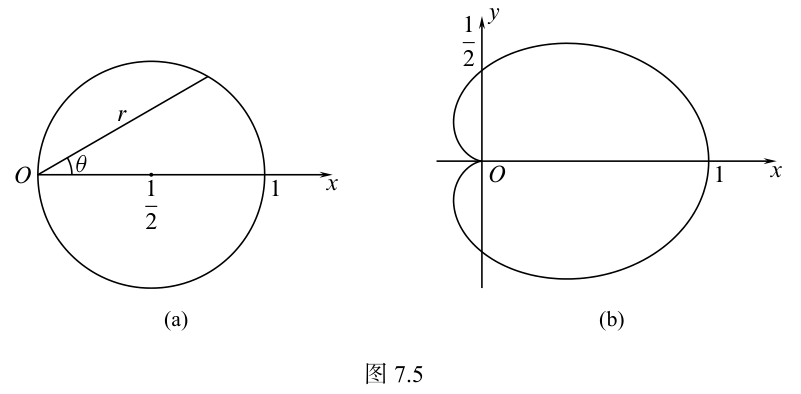
\includegraphics{public/figures/complex-functions/ch07-fig-7-5.png}

\subsection*{边界条件的适用范围}\label{ch07-s3-heading-5}

Jordan
条件用于把细小的横截弧变成细小的边界侧，并排除边界粘合。一般单连通域仅由
Riemann
定理不能推出闭包同胚。下一节对有界简单多边形可直接使用本节定理；出现裂缝或多个无穷远``端''时，则须按到达侧区分边界，而不能将所有端看成同一个边界参数。

\section{Schwarz–Christoffel 公式}
对应教材第 223---234 页。Riemann
映射定理保证映射存在，本节利用直边的反射和角点的局部幂次，把存在性转成积分公式。除特别说明外，多边形是有界简单多边形，顶点沿边界正向排列；``全纯映射''取有限值，``单叶亚纯映射''允许域内有一个对应球面无穷远的极点。

\subsection*{定理索引}\label{ch07-s4-heading-1}

\hyperref[ch07-s4-heading-2]{引理 7.4.1} · \hyperref[ch07-s4-heading-3]{引理 7.4.2} ·
\hyperref[ch07-s4-heading-4]{定理 7.4.3} · \hyperref[ch07-s4-heading-5]{定理 7.4.4} ·
\hyperref[ch07-s4-heading-6]{定理 7.4.5} · \hyperref[ch07-s4-heading-7]{定理 7.4.6} ·
\hyperref[ch07-s4-heading-8]{例 7.4.7} · \hyperref[ch07-s4-heading-9]{例 7.4.8} ·
\hyperref[ch07-s4-heading-10]{例 7.4.9} ·
\hyperref[ch07-s4-heading-11]{公式的使用顺序与全章联系}

\Needspace{8\baselineskip}
\subsection{引理 7.4.1：上半平面到多边形的边界映射}\label{ch07-s4-heading-2}

存在双全纯映射 \(f:\mathbb H\to G\)，连续延拓为
\(\mathbb H\cup\mathbb R\cup\{\infty\}\) 到 \(\overline G\)
的同胚，边界正向对应。

证明：取 \(a\in\mathbb H\)，分式线性变换 \(T(z)=(z-a)/(z-\bar a)\) 将
\(\mathbb H\) 映到 \(\mathbb D\)，将扩充实轴
\(\widehat{\mathbb R}=\mathbb R\cup\{\infty\}\) 一一映到圆周。将它与定理
7.2.1、7.3.1 给出的闭圆盘到闭多边形的映射复合即可。

教材只写``实轴一一映为整个边界''时应补上
\(\infty\)；普通实轴的像实际缺少 \(f(\infty)\)。可预复合一个实 Möbius
自同构，使 \(f(\infty)\) 落在边的内部，于是所有顶点的原像
\(a_1,\ldots,a_n\) 都有限。这是定理 7.4.3 采用的归一化；定理 7.4.5
再处理顶点原像等于 \(\infty\) 的情形。

\Needspace{8\baselineskip}
\subsection{引理 7.4.2：角点处的幂次展开}\label{ch07-s4-heading-3}

设 \(w_0\) 是边界由两条直线段构成的角点，域内角为
\(\alpha\pi\)，\(0<\alpha<2\)。设双全纯映射 \(f\)
在相应边界邻域连续且一一，\(f(z_0)=w_0\)，\(z_0\in\mathbb R\)。则在上半平面侧的充分小邻域内

\[
f(z)=w_0+(z-z_0)^\alpha\bigl(c_0+c_1(z-z_0)+\cdots\bigr),\quad c_0\ne0.
\qquad\text{(7.4.1)}
\]

证明：先平移旋转，使角域为
\(0<\arg(w-w_0)<\alpha\pi\)。只在这个局部扇形取
\((w-w_0)^{1/\alpha}\)，将其化为上半平面。复合后得到
\(u(z)\)，它把边界小线段一一映到实线段，内部映到同一上侧。Schwarz 反射使
\(u\)
全纯延到整个小圆盘；上、下两侧的像在相反半平面，边界单射，故延拓仍局部单射。因此
\(u'(z_0)\ne0\)，有

\[
u(z)=(z-z_0)b(z),\qquad b(z_0)\ne0.
\]

缩小圆盘使 \(b\) 无零点，取其全纯对数并令
\(h=b^\alpha\)。把旋转常数吸收入 \(h\)，得
\(f-w_0=(z-z_0)^\alpha h(z)\)，其中 \(h\) 全纯且
\(h(z_0)\ne0\)，展开即得结论。

这里 \(b_1\ne0\) 依赖反射后仍单射，不能仅从域内 \(f'\ne0\)
推到边界。幂函数只须在局部角域取分支；没有理由在任意原域中直接选一个全局角坐标。

\Needspace{8\baselineskip}
\subsection{定理 7.4.3：Schwarz--Christoffel 公式}\label{ch07-s4-heading-4}

设 \(f:\mathbb H\to G\) 双全纯，\(G\) 的正向顶点为 \(w_k\)，内角为
\(\alpha_k\pi\)，\(0<\alpha_k<2\)；假设顶点原像 \(a_k=f^{-1}(w_k)\)
全为有限实数。则存在 \(C\ne0,C_1\in\mathbb C\)，对固定
\(z_0\in\mathbb H\) 有

\[
f(z)=C\int_{z_0}^z\prod_{k=1}^n(\zeta-a_k)^{\alpha_k-1}\,d\zeta+C_1.
\qquad\text{(7.4.5)}
\]

各因子规定 \(0<\arg(\zeta-a_k)<\pi\)；路径在 \(\mathbb H\)
中。被积函数在单连通域 \(\mathbb H\)
全纯，所以积分与路径无关。换用其他一致分支只改变非零乘常数 \(C\)。

证明：令 \(q=f''/f'\)，域内因单叶性有
\(f'\ne0\)。在每个顶点原像以外的实区间，\(f\)
的边界值落在一条直线上，故可沿该区间反射。若直线方向为
\(\theta\)，下半平面的延拓形如
\(A+e^{2i\theta}\overline{f(\bar z)}\)，因而其二阶导数与一阶导数之比恒为
\(\overline{q(\bar z)}\)，与所选边无关。边界局部反射保持单射，导数不为零。所以这些商拼成
\(\mathbb C\setminus\{a_k\}\) 上的一个全纯函数。

由引理 7.4.2，\(f-w_k=(z-a_k)^{\alpha_k}h_k(z)\)，\(h_k(a_k)\ne0\)。于是

\[
\begin{aligned}
f'(z)&=(z-a_k)^{\alpha_k-1}Q_k(z),\quad Q_k(a_k)=\alpha_kh_k(a_k)\ne0,\\
q(z)&=\frac{\alpha_k-1}{z-a_k}+\frac{Q_k'(z)}{Q_k(z)}.
\end{aligned}\qquad\text{(7.4.6)}
\]

故 \(q\) 在 \(a_k\) 至多有单极点，留数为 \(\alpha_k-1\)。若
\(\alpha_k=1\)，该点可去；教材``都是一阶极点''须排除这一平角情形。

因为 \(f(\infty)\) 位于直边内部，以 \(t=-1/z\)
作边界局部坐标并反射，局部单射给出

\[
f(z)=b_0+b_1z^{-1}+O(z^{-2}),\quad b_1\ne0,
\qquad q(z)=-2z^{-1}+O(z^{-2}).
\]

于是整函数 \(q(z)-\sum_k(\alpha_k-1)/(z-a_k)\) 在无穷远趋于零，由
Liouville 定理恒零。在 \(\mathbb H\) 上，\(f'\)
无零点，有全纯对数，故积分得到

\[
\frac{f''(z)}{f'(z)}=\sum_{k=1}^n\frac{\alpha_k-1}{z-a_k},\qquad
f'(z)=C\prod_{k=1}^n(z-a_k)^{\alpha_k-1}.
\]

再积分得到式（7.4.5）。由于
\(\alpha_k>0\)，角点附近原函数的积分收敛；又由多边形内角和
\(\sum\alpha_k=n-2\)，无穷远处被积函数为 \(O(z^{-2})\)，与有限的
\(f(\infty)\) 相符。

这个公式是已存在的多边形映射必须满足的形式。任取预顶点 \(a_k\)
与角参数所写的积分，不会自动产生指定边长的多边形；还须解出预顶点位置并核对边界与单叶性。

\Needspace{8\baselineskip}
\subsection{定理 7.4.4：三个有序边界点的归一化}\label{ch07-s4-heading-5}

设 \(a_1<a_2<a_3\) 为三个实数，\(w_1,w_2,w_3\)
是多边形边界按正向循环排列的三个不同顶点。存在唯一双全纯映射
\(f:\mathbb H\to G\)，连续到扩充边界且满足 \(f(a_j)=w_j\)。

证明：任取引理 7.4.1 的映射 \(\phi\)，令
\(b_j=\phi^{-1}(w_j)\in\widehat{\mathbb R}\)。两组三点具有相同的循环顺序。分别用交比把三点送到
\(0,1,\infty\)，再复合，得到唯一实 Möbius 变换 \(T\)，满足
\(T(a_j)=b_j\)。循环顺序相同使其行列式为正；由

\[
\operatorname{Im}\frac{Az+B}{Cz+D}
=\frac{(AD-BC)\operatorname{Im}z}{|Cz+D|^2}
\]

知 \(T(\mathbb H)=\mathbb H\)。于是 \(f=\phi\circ T\) 满足要求。若另有
\(g\)，则 \(g^{-1}\circ f\)
是上半平面自同构，化到圆盘后由第四章自同构分类知它是 Möbius
变换；固定三个不同边界点只能是恒等，故 \(f=g\)。

循环顺序不可去掉。无穷远也可作为这三点之一；循环顺序并不等同于把含无穷远的三点机械地写成通常大小次序。

\Needspace{8\baselineskip}
\subsection{定理 7.4.5：一个预顶点在无穷远}\label{ch07-s4-heading-6}

若 \(a_n=\infty\)，其余预顶点有限，则

\[
f(z)=C\int_{z_0}^z\prod_{k=1}^{n-1}(\zeta-a_k)^{\alpha_k-1}\,d\zeta+C_1.
\qquad\text{(7.4.8)}
\]

证明：选 \(a<\min_{k<n}a_k\)，令 \(T(z)=1/(a-z)\)，它保持上半平面，将
\(a_n=\infty\) 送到 \(b_n=0\)，并使所有预顶点有限。对
\(F=f\circ T^{-1}\) 用定理 7.4.3。设 \(\tau=T(\zeta)\)，则

\[
\tau-b_k=\frac{\zeta-a_k}{(a-\zeta)(a-a_k)},\qquad
\tau=\frac1{a-\zeta},\qquad d\tau=\frac{d\zeta}{(a-\zeta)^2}.
\]

变换后的 \(a-\zeta\) 总指数是

\[
-\sum_{k=1}^{n}(\alpha_k-1)-2=0.
\]

各固定因子及分支常数并入 \(C\)，便得到结论。在无穷远，被积函数为
\(O(z^{-1-\alpha_n})\)，原函数与 \(w_n\) 之差为
\(O(z^{-\alpha_n})\)，恰与角点展开在坐标 \(-1/z\) 下相合。

\Needspace{8\baselineskip}
\subsection{定理 7.4.6：无穷远顶点与平行端}\label{ch07-s4-heading-7}

对由有限条直线段、射线组成的单连通多边形域，把同一球面无穷远处不同的到达端分别计为边界顶点。若一个端在远处是张角
\(\beta\pi\) 的扇形，规定其角参数
\(\alpha=-\beta\)；若是两条平行边夹成的半带端，规定
\(\alpha=0\)。以这种角参数，Schwarz--Christoffel
公式仍成立。相同几何裂缝的两侧须分别计为边；有限裂缝端点允许内角
\(2\pi\)，角点证明仍用局部开方化直。本断言讨论内部不取 \(\infty\)
的全纯映射。

证明：先说明所用边界概念。沿每个端作一条横截线，将有限条边、裂缝的两侧及各端按边界行进次序分别记录，补成一个抽象边界圆周。有限角处用局部扇形坐标，非平行无限端以交点
\(b\) 为中心用 \(1/(w-b)\)
再开幂，平行端用指数坐标，均得到半圆盘边界邻域。有限多条边没有累积，横截线切下的核心由
Jordan
定理给出闭圆盘，重新接上各半圆盘领圈仍为闭圆盘。这就是此处的边界闭包；多个端可代表同一个球面点，但在这个闭包中不同。

Riemann 映射连续到这个边界的证明与定理 7.3.1
相同：在上述有限个坐标邻域取一个光滑正度量，核心上补齐，使补成的闭圆盘成为有限面积的紧曲面。拉回这个度量后，式（7.3.1）中的积分等于目标的有限度量面积，式（7.3.2）及小横截弧论证逐字成立。边界粘合反证在目标的局部半圆盘坐标中用反射，同样成立。因此每个边和端有一个确定的边界原像，且局部边界映射单射。这里仅把已有的长度---面积证明放到有限个坐标中，不假定一般域的原端定理。

在有限角点，式（7.4.6）仍成立。对非平行无限端，作 \(v=1/(f-b)\)。端在
\(v=0\) 处的角为 \(\beta\pi\)，由角点展开

\[
v=(z-a)^\beta h(z),\quad h(a)\ne0,
\qquad f=b+(z-a)^{-\beta}/h(z).
\]

故 \(f'=(z-a)^{-\beta-1}Q(z)\)、\(Q(a)\ne0\)，从而 \(f''/f'\) 的留数是
\(-\beta-1=\alpha-1\)。

对宽为 \(d\) 的平行半带端，适当平移旋转后，\(v=\exp(\pm\pi(f-b)/d)\)
把该端化为 \(v=0\) 附近的半圆盘。反射及局部单射说明
\(v=(z-a)h(z)\)、\(h(a)\ne0\)，所以

\[
f=b\pm\frac d\pi\bigl(\log(z-a)+\log h(z)\bigr).
\]

\(f'\) 为具有非零留数的单极点，\(f''/f'\) 的留数为 \(-1=\alpha-1\)，对应
\(\alpha=0\)。这也解释了无限端出现对数而不是把 \(0\) 次幂误看成常数。

先归一化使 \(f(\infty)\) 为有限直边内点。跨每条直边反射后，\(f''/f'\)
仍拼成单值函数；减去以上有限个主部，所得整函数在无穷远趋零，故恒零，积分即得公式。如有一个预顶点在
\(\infty\)，用前一定理的变量代换；总角关系 \(\sum(\alpha_k-1)=-2\)
也可直接比较 \(f''/f'\) 在无穷远的 \(-2/z\) 系数得到。

\noindent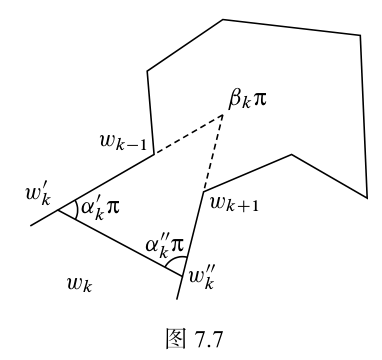
\includegraphics{public/figures/complex-functions/ch07-fig-7-7.png}

教材采用``将截线移到无穷远''的直观推导，但仅让端点形式趋近不足以证明映射及导数收敛。以上用局部角坐标和对数导数给出证明，并单独包含平行端。若映射在域内取
\(\infty\)，它是亚纯映射，必须另外加入内部极点产生的因子，见习题校注。

\Needspace{8\baselineskip}
\subsection{例 7.4.7：上半平面到三角形}\label{ch07-s4-heading-8}

设三角形正向顶点为 \(w_1,w_2,w_3\)，内角为
\(\alpha_1\pi,\alpha_2\pi,\alpha_3\pi\)，\(\alpha_1+\alpha_2+\alpha_3=1\)。规定
\(0,1,\infty\) 依次映到这三个顶点。

解：令

\[
f(z)=w_1+\frac{w_2-w_1}{B(\alpha_1,\alpha_2)}
\int_0^z\zeta^{\alpha_1-1}(1-\zeta)^{\alpha_2-1}\,d\zeta.
\qquad\text{(7.4.9)}
\]

在 \(\mathbb H\) 规定
\(0<\arg\zeta<\pi\)、\(-\pi<\arg(1-\zeta)<0\)，故在 \(0<x<1\)
上的上侧极限为正实数。下限 \(0\) 按边界极限理解，因 \(\alpha_1>0\)
可积；同理 \(1\) 附近可积，无穷远的指数为 \(-1-\alpha_3<-1\)。

由定理 7.4.4 存在唯一归一化三角形映射，它由定理 7.4.5
必有上述被积形式。代入 \(f(0)=w_1,f(1)=w_2\)
唯一确定两个常数，因而式（7.4.9）正是所求映射，第三顶点及单叶性已由存在性与唯一性保证。

教材还给出

\[
B(\alpha_1,\alpha_2)
=\frac{\Gamma(\alpha_1)\Gamma(\alpha_2)}{\Gamma(1-\alpha_3)}
=\frac{\Gamma(\alpha_1)\Gamma(\alpha_2)\Gamma(\alpha_3)\sin(\pi\alpha_3)}\pi.
\]

为说明这一步的依据，对 \(p,q>0\) 在 \(\Gamma(p)\Gamma(q)\)
的正二重积分中作 \(x=rt,y=r(1-t)\)，Jacobian 为 \(r\)，得到
\(\Gamma(p)\Gamma(q)=\Gamma(p+q)B(p,q)\)。又对
\(0<s<1\)，\(B(s,1-s)=\int_0^\infty t^{s-1}/(1+t)\,dt\)。取
\(0<\arg z<2\pi\) 的钥匙孔围道，内外圆积分分别因 \(s>0,s<1\)
趋零，正轴两侧积分为 \((1-e^{2\pi is})B(s,1-s)\)，留数为
\(e^{i\pi(s-1)}\)，于是 \(B(s,1-s)=\pi/\sin\pi s\)。这就补证了此处使用的
Beta--Gamma 关系和余元公式。

\Needspace{8\baselineskip}
\subsection{例 7.4.8：上半平面到半带}\label{ch07-s4-heading-9}

求 \(\mathbb H\) 到
\(G=\{w:-\pi/2<\operatorname{Re}w<\pi/2,\ \operatorname{Im}w>0\}\)
的保角映射。

解：有限角为 \(\pi/2,\pi/2\)，无穷远平行端的角参数为 \(0\)。取预顶点
\(-1,1,\infty\)，得 \(f'(z)=1/\sqrt{1-z^2}\)，其中平方根是 \(\mathbb H\)
中在 \((-1,1)\) 上侧取正实值的全纯分支。因此

\[
f(z)=\int_0^z\frac{d\zeta}{\sqrt{1-\zeta^2}}=\arcsin z.
\]

下限按边界极限，\(f(-1)=-\pi/2,f(1)=\pi/2\)。为核查映射范围，令
\(w=u+iv\in G\)，则 \(\operatorname{Im}\sin w=\cos u\sinh v>0\)。若
\(\sin w_1=\sin w_2\)，则 \(w_1-w_2\in2\pi\mathbb Z\) 或
\(w_1+w_2\in\pi+2\pi\mathbb Z\)；半带条件使前者仅能为零，后者不可能。故
\(\sin\) 在 \(G\) 单叶。

它还是到 \(\mathbb H\)
的适当映射：\(|\sin(u+iv)|^2=\sin^2u+\sinh^2v\)，所以当 \(v\to\infty\)
时像趋无穷；接近三条有限边时像趋实轴。任意 \(\mathbb H\)
中紧集的原像因而紧。适当性使像在 \(\mathbb H\)
中闭，开映射定理使它开；由连通性知像为整个 \(\mathbb H\)。其逆即上述
\(\arcsin\) 分支。

\noindent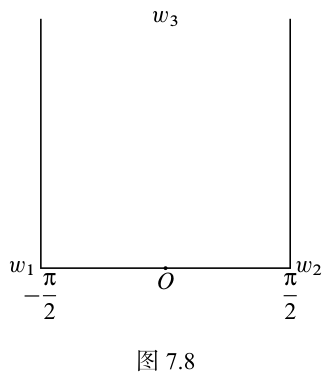
\includegraphics{public/figures/complex-functions/ch07-fig-7-8.png}

\Needspace{8\baselineskip}
\subsection{例 7.4.9：带状域到带有无限端的多边形}\label{ch07-s4-heading-10}

设 \(h>0\)，先取 \(0<\beta<1\)。教材图 7.9 的目标域由两条在 \(\pm ih\)
拐弯的边界围成：左端为宽 \(2h\) 的水平带，右端向外张开。先处理上半部分
\(G'\)；它有一个平行端、一个张角 \(\beta\pi\) 的无限端和内角
\((1+\beta)\pi\) 的角点 \(ih\)。

图 7.9 左侧下边界的印刷标记应为 \(-\pi i\)，源域以正文所列
\(-\pi<\operatorname{Im}z<\pi\) 为准。

\noindent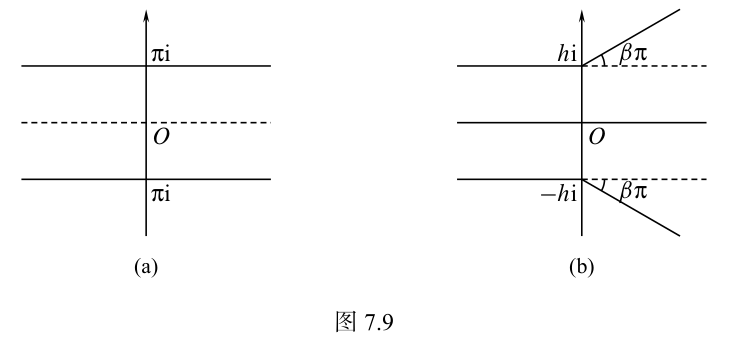
\includegraphics{public/figures/complex-functions/ch07-fig-7-9.png}

解：\(\zeta=e^z\) 将 \(0<\operatorname{Im}z<\pi\) 双全纯地映为
\(\mathbb H\)。三个角参数依次为 \(0,-\beta,1+\beta\)，取对应预顶点
\(0,\infty,-1\)，得

\[
F(\zeta)=\frac h\pi\int_{-1}^{\zeta}\frac{(1+t)^\beta}{t}\,dt+ih.
\qquad\text{(7.4.13)}
\]

规定 \(0<\arg(1+t)<\pi\)，路径由 \(-1\) 的上侧出发并留在
\(\mathbb H\)，不得穿越 \(t=0\)。因 \(\beta>-1\)，下端积分收敛。原函数在
\(\mathbb H\) 唯一，边界下限由极限确定。

说明系数如何决定。一般式的系数先记作 \(C\)；在 \((-1,0)\)
上被积函数为负实数，像沿水平边从 \(ih\) 向左走，因此 \(C\) 为正实数。取
\(t=\rho e^{i\theta}\) 的小上半圆，从 \(-\rho\) 顺时针走到 \(\rho\)，有

\[
\int_{-\rho}^{\rho}\frac{(1+t)^\beta}{t}\,dt=-\pi i+O(\rho).
\]

对应两条水平边的虚部差是 \(-h\)，故 \(C\pi=h\)，即
\(C=h/\pi\)；这同时给出正实轴上 \(\operatorname{Im}F=0\)。

对于 \(t<-1\)
的上侧，\((1+t)^\beta=|1+t|^\beta e^{i\beta\pi}\)，沿该边的积分形成从
\(ih\) 向右上方发出的射线；\(t\to0\) 给平行端，\(t\to\infty\) 给张角
\(\beta\pi\) 的右端。定理 7.4.6
保证存在的归一化映射必有此形式，三个边界位置与宽度决定常数，故它是所需双全纯映射。

于是 \(W(z)=F(e^z)\) 映上半带到 \(G'\)。在 \(\operatorname{Im}z=0\) 上
\(W\) 为实数，作 Schwarz 反射得到整个 \(-\pi<\operatorname{Im}z<\pi\)
上的映射。上、下半带的像分别位于实轴上、下，实轴映射单射且导数为正，故反射后的映射仍单叶并满射到图示目标。

当
\(\beta=1\)，角点成为裂缝端点，须把裂缝两侧分别记为边；局部开方化直后，前述边界与公式论证仍适用。积分得到

\[
F(\zeta)=\frac h\pi(\operatorname{Log}\zeta+\zeta+1),\qquad
W(z)=\frac h\pi(e^z+z+1).
\]

它将带状域映为

\[
\mathbb C\setminus\bigl(\{x+ih:x\le0\}\cup\{x-ih:x\le0\}\bigr).
\]

必须删去两个端点 \(\pm ih\) 才是开域；教材文字写 \(x<0\)
时漏掉端点，与其图形和开映射性质不合。

\noindent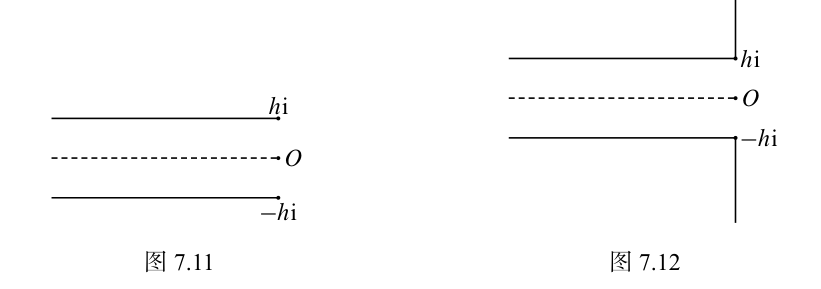
\includegraphics{public/figures/complex-functions/ch07-fig-7-11-12.png}

当 \(\beta=1/2\)，令 \(u=\sqrt{1+\zeta}\)，在 \(\mathbb H\) 取
\(\operatorname{Re}u>0,\operatorname{Im}u>0\) 的根。由 \(d\zeta=2u\,du\)
直接积分可得

\[
F(\zeta)=\frac{2h}{\pi}\left[u+\operatorname{Log}(u-1)-\frac12\operatorname{Log}\zeta\right],
\]

其中 \(\operatorname{Log}\zeta\) 与 \(\operatorname{Log}(u-1)\)
均取虚部在 \((0,\pi)\) 的分支；当 \(\zeta\to-1\) 上侧时，右端趋于
\(ih\)。代入 \(\zeta=e^z\) 时，在上半带有
\(\operatorname{Log}(e^z)=z\)；延拓到整带应使用由此确定的同一个全纯分支，不能逐点重新选择主值。因此

\[
W(z)=\frac{2h}{\pi}\left[\sqrt{1+e^z}
+\log\bigl(\sqrt{1+e^z}-1\bigr)-\frac z2\right].
\]

平方根在带内以实轴上正根确定，对数在实轴上取实值并全纯接续。此时目标是水平带在右侧打开后的域，边界为两条从左无穷远到
\(\pm ih\)、再分别竖直走向上下无穷远的折线，如图 7.12。

\subsection*{公式的使用顺序与全章联系}\label{ch07-s4-heading-11}

先判断目标是 Jordan
多边形、含裂缝的域，还是球面外域；再按边界次序记录角参数及预顶点，标出哪一个预顶点在
\(\infty\)。固定三个有序边界点后，写出各因子的分支，用边长、宽度或指定值确定常数。最后核验端点积分、无穷远渐近、边界次序及单叶性。

本章的逻辑是：局部一致有界经 Cauchy
估计变成紧性，紧性使归一化导数极值达到，平方根构造迫使极值映射满射，Jordan
边界条件再使它成为闭域同胚，直边反射和角点幂次最终给出积分公式。第八章将使用这些映射，把调和函数及边值问题搬到圆盘和上半平面。

\clearpage\section*{第七章习题}\phantomsection\addcontentsline{toc}{section}{第七章习题}
按上传教材第 213、217---218、222、234 页收录，共 25
道主编号题：7＋7＋5＋6。本书本章没有另设章末复习题。以下保留原题条件、小问和教材自带的括号提示，不附常规解答。原题疑义另列于最后的校注，不把修订文字混入原题。

\subsection*{习题索引}\label{ch07-practice-heading-1}

\hyperref[ch07-practice-heading-2]{习题 7.1} · \hyperref[ch07-practice-heading-3]{习题 7.2} ·
\hyperref[ch07-practice-heading-4]{习题 7.3} · \hyperref[ch07-practice-heading-5]{习题 7.4} ·
\hyperref[ch07-practice-heading-6]{原题校注}

\Needspace{8\baselineskip}
\subsection{习题 7.1}\label{ch07-practice-heading-2}

\hyperref[ch07-s1-heading-9]{本节七题详解}

\par\Needspace{5\baselineskip}
\noindent\textbf{1.} 设 \(\{f_n\}\) 是域 \(D\) 上的全纯函数列，并且在 \(D\)
上内闭一致有界。证明：若 \(\lim_{n\to\infty}f_n(z)\) 在 \(D\)
上处处存在，则 \(\{f_n\}\) 在 \(D\) 上内闭一致收敛。

\par\Needspace{5\baselineskip}
\noindent\textbf{2.} 设 \(\{f_n\}\) 是域 \(D\) 上的全纯函数列，并且在 \(D\)
上内闭一致有界，\(A=\{z=x+iy\in D:x,y\text{ 为有理数}\}\)。证明：若
\(\lim_{n\to\infty}f_n(z)\) 在 \(A\) 上处处存在，则 \(\{f_n\}\) 在 \(D\)
上内闭一致收敛。

\par\Needspace{5\baselineskip}
\noindent\textbf{3.} （Vitali 定理）设 \(\{f_n\}\) 是域 \(D\)
上的全纯函数列，并且在 \(D\) 上内闭一致有界，\(\{z_n\}\) 是 \(D\)
中彼此不同的点列，\(\lim_{n\to\infty}z_n=z_0\in D\)。证明：若
\(\lim_{n\to\infty}f_n(z)\) 在 \(\{z_n\}\) 上处处存在，则 \(\{f_n\}\) 在
\(D\) 上内闭一致收敛。

\par\Needspace{5\baselineskip}
\noindent\textbf{4.} 设 \(\mathcal F\) 是域 \(D\)
上的全纯函数族，\(z_0\in D\)。证明：若

（1）\(\operatorname{Re}f(z)\ge0,\ \forall z\in D,\ f\in\mathcal F\)；

（2）\(f(z_0)=g(z_0),\ \forall f,g\in\mathcal F\)，

则 \(\mathcal F\) 是 \(D\) 上的正规族。并举例说明条件（2）是不可去掉的。

\par\Needspace{5\baselineskip}
\noindent\textbf{5.} 设 \(\mathcal F\) 是域 \(D\) 上的正规全纯函数族，\(g\)
是整函数。证明：\(\{g\circ f:f\in\mathcal F\}\) 也是 \(D\) 上的正规族。

\par\Needspace{5\baselineskip}
\noindent\textbf{6.} 设 \(D\) 是有界域，\(0<M<\infty\)。证明：

\[
\mathcal F=\left\{f\in H(D):\iint_D|f(z)|^2\,dx\,dy\le M\right\}
\]

是 \(D\) 上的正规族。

\par\Needspace{5\baselineskip}
\noindent\textbf{7.} 设 \(\{f_n\}\) 是域 \(D\) 上的全纯函数列，并且在 \(D\)
上内闭一致有界。证明：若存在 \(z_0\in D\)，使得
\(\lim_{n\to\infty}f_n(z_0)=A\) 存在，并且
\(f_n(D)\subset\mathbb C\setminus\{A\}\)（\(n\in\mathbb N\)），则
\(\{f_n\}\) 在 \(D\) 上内闭一致收敛于常数 \(A\)。

\Needspace{8\baselineskip}
\subsection{习题 7.2}\label{ch07-practice-heading-3}

\par\Needspace{5\baselineskip}
\noindent\textbf{1.} （推广的 Liouville 定理）设 \(D\) 是异于 \(\mathbb C\)
的单连通域。证明：若 \(f\) 是整函数，并且 \(f(\mathbb C)\subset D\)，则
\(f\) 是常值函数。

\par\Needspace{5\baselineskip}
\noindent\textbf{2.} 设 \(D\) 是异于 \(\mathbb C\)
的单连通域，\(a\in D\)。证明：若 \(f\) 将 \(D\) 双全纯地映为
\(B(0,1)\)，并且 \(f(a)=0,f'(a)>0\)，则

\[
\min_{z\in\partial D}|z-a|\le\frac1{f'(a)}\le\max_{z\in\partial D}|z-a|.
\]

称 \(1/f'(a)\) 为 \(D\) 在 \(a\) 处的映射半径。

\par\Needspace{5\baselineskip}
\noindent\textbf{3.} 设 \(D\) 是异于 \(\mathbb C\) 的单连通域，\(a\in D\)，\(f\)
将 \(D\) 双全纯地映为 \(B(0,1)\)，并且 \(f(a)=0,f'(a)>0\)。证明：若
\(g\) 将 \(D\) 双全纯地映为 \(B(0,1)\)，\(p=g^{-1}(0)\)，则

\[
g(z)=\frac{g'(a)}{|g'(a)|}\frac{f(z)-f(p)}{1-\overline{f(p)}f(z)}.
\]

\par\Needspace{5\baselineskip}
\noindent\textbf{4.} 设 \(D\) 为异于 \(\mathbb C\)
的凸域，\(a\in D\)，\(\mathcal F=\{f\in H(D):f(a)=0,f'(a)>0\}\)。证明：\(\mathcal F\)
中满足 \(f(D)=B(0,1)\) 和
\(\operatorname{Re}f'(z)>0\)（\(\forall z\in D\)）的 \(f\)
最多只有一个。

\par\Needspace{5\baselineskip}
\noindent\textbf{5.} 设 \(D\) 是异于 \(\mathbb C\) 的单连通域，\(a\in D\)，\(R\)
为 \(D\) 在 \(a\) 处的映射半径。证明：若
\(F\in H(D)\)，\(F(a)=0,F'(a)=1\)，则
\(\sup_{z\in D}|F(z)|\ge R\)。等号成立当且仅当 \(F\) 是将 \(D\) 映为
\(B(0,R)\) 的双全纯映射。

\par\Needspace{5\baselineskip}
\noindent\textbf{6.} 证明：

（1）存在 \(B(0,1)\) 上的全纯函数 \(f\)，使得 \(f(B(0,1))=\mathbb C\)；

（2）对于 \(a\in\mathbb C\)，存在 \(B(0,1)\) 上的全纯函数 \(f\)，使得
\(f(B(0,1))=\mathbb C\setminus\{a\}\)。

并将这里的结论与习题 6.3 的第 3 题和第 4 题作比较。

\par\Needspace{5\baselineskip}
\noindent\textbf{7.} 设 \(D\) 是异于 \(\mathbb C\) 的单连通域，\(a\in D\)，\(R\)
为 \(D\) 在 \(a\) 处的映射半径。证明：若
\(F\in H(D)\)，\(F(a)=0,F'(a)=1\)，则

\[
\iint_D|F'(z)|^2\,dx\,dy\ge\pi R^2.
\]

等号成立当且仅当 \(F\) 是将 \(D\) 映为 \(B(0,R)\) 的双全纯映射。

\Needspace{8\baselineskip}
\subsection{习题 7.3}\label{ch07-practice-heading-4}

\par\Needspace{5\baselineskip}
\noindent\textbf{1.} 利用 Schwarz 对称原理和边界对应定理证明：将 \(B(0,1)\)
映为自身的双全纯映射一定是分式线性变换。

\par\Needspace{5\baselineskip}
\noindent\textbf{2.} 证明：若 \(f\) 将圆环 \(\{z\in\mathbb C:r_1<|z|<r_2\}\)
双全纯地映为圆环 \(\{w\in\mathbb C:R_1<|w|<R_2\}\)，则 \(f\) 将闭圆环
\(\{z\in\mathbb C:r_1\le|z|\le r_2\}\) 同胚地映为闭圆环
\(\{w\in\mathbb C:R_1\le|w|\le R_2\}\)。

\par\Needspace{5\baselineskip}
\noindent\textbf{3.} 设 \(D\)
是由简单闭曲线所围成的单连通域，\(z_1,z_2,z_3\in\partial D\)
是彼此不同的三点，按 \(\partial D\) 的正向排列。证明：若
\(w_1,w_2,w_3\in\partial B(0,1)\) 是彼此不同的三点，按
\(\partial B(0,1)\) 的正向排列，则存在唯一的 \(\varphi\)，将 \(D\)
双全纯地映为 \(B(0,1)\)，将 \(\overline D\) 同胚地映为
\(\overline{B(0,1)}\)，并且 \(f(z_k)=w_k,\ k=1,2,3\)。

\par\Needspace{5\baselineskip}
\noindent\textbf{4.} （边界对应原理）设 \(D\) 是由简单闭曲线 \(\gamma\)
所围成的单连通域（\(\gamma\)
不必可求长），\(f\in H(D)\cap C(\overline D)\)。证明：若 \(f\) 将
\(\gamma\) 一一地映为简单闭曲线 \(\Gamma\)，则 \(f\) 将 \(D\)
双全纯地映为由 \(\Gamma\) 所围成的单连通域 \(G\)。将这里的结论与习题 4.4
中的第 17 题作比较。

\par\Needspace{5\baselineskip}
\noindent\textbf{5.} 设 \(f\in H(B(0,1))\)，\(f(0)=0,f'(0)=a>0\)。证明：若
\(f(B(0,1))\subset B(0,1)\)，则 \(f\) 在

\[
B\left(0,\frac{a}{1+\sqrt{1-a^2}}\right)
\]

上双全纯。

\Needspace{8\baselineskip}
\subsection{习题 7.4}\label{ch07-practice-heading-5}

\par\Needspace{5\baselineskip}
\noindent\textbf{1.} 设
\(L_k=\{z=re^{2k\pi i/n}:1\le r<\infty\}\)，\(G=\mathbb C\setminus\bigl(\bigcup_{k=1}^nL_k\bigr)\)。求出将上半平面映为
\(G\) 的双全纯映射 \(\varphi\)，使得 \(\varphi(i)=0\)。

教材括号提示：

\[
\varphi(z)=\frac{z^2+1}{\left(\displaystyle\sum_{k=0}^{\lfloor n/2\rfloor}(-1)^k\binom n{2k}z^{n-2k}\right)^{2/n}}.
\]

\par\Needspace{5\baselineskip}
\noindent\textbf{2.} 证明：将 \(B(0,1)\) 映为 \(n\) 角形内部的双全纯映射
\(\varphi\) 具有形状

\[
\varphi(z)=C_0\int_{z_0}^z\prod_{k=1}^n(\zeta-a_k)^{\alpha_k-1}\,d\zeta+C_1,
\]

其中，\(a_1,\ldots,a_n\in\partial B(0,1)\) 是与该 \(n\)
角形顶点相对应的点；\(\alpha_1\pi,\ldots,\alpha_n\pi\) 是该 \(n\)
角形的内角；\(z_0\in B(0,1)\)。

\par\Needspace{5\baselineskip}
\noindent\textbf{3.} 设 \(G\) 是正 \(n\) 角形，\(O\) 是它的中心，\(1\)
是它的一个顶点。求出将 \(B(0,1)\) 映为 \(G\) 的双全纯映射
\(\varphi\)，使得 \(\varphi(0)=0,\varphi'(0)>0\)。

教材括号提示：

\[
\varphi(z)=\frac{n}{B(1/n,1-2/n)}\int_0^z(1-\zeta^n)^{-2/n}\,d\zeta.
\]

\par\Needspace{5\baselineskip}
\noindent\textbf{4.} 证明：将上半平面映为 \(\mathbb C_\infty\) 中的 \(n\)
角形外部的单叶亚纯函数 \(\varphi\) 具有形状

\[
\varphi(z)=C_0\int_{z_0}^z\prod_{k=1}^n(\zeta-a_k)^{\alpha_k-1}
\frac1{(\zeta-a_0)(\zeta-\bar a_0)}\,d\zeta+C_1,
\]

其中，\(a_1,\ldots,a_n\in\mathbb R\) 是与该 \(n\)
角形顶点相对应的点；\(\alpha_1\pi,\ldots,\alpha_n\pi\) 是该 \(n\)
角形的外角；\(a_0=\varphi^{-1}(\infty)\)，\(\operatorname{Im}z_0>0\)。

\par\Needspace{5\baselineskip}
\noindent\textbf{5.} 设

\[
G=\mathbb C_\infty\setminus\bigl([0,1]\cup[0,e^{2\pi i/3}]\cup[0,e^{-2\pi i/3}]\bigr),
\]

\(\operatorname{Im}z_0>0\)。求出将上半平面映为 \(G\) 的单叶亚纯映射
\(\varphi\)，使得 \(\varphi(z_0)=\infty\)。

教材括号提示（原样保留）：

\[
\varphi(z)=\frac{\bigl[(z-z_0)^3-3y_0^2(z-x_0)\bigr]^{2/3}}{(z-x_0)^2+y_0^2}.
\]

\par\Needspace{5\baselineskip}
\noindent\textbf{6.} 设 \(L_1,\ldots,L_n\) 是以 \(O\) 为端点的 \(n\)
条线段，它们彼此仅在 \(O\)
处相交，\(\operatorname{Im}a_0>0\)。证明：将上半平面映为
\(G=\mathbb C_\infty\setminus\bigl(\bigcup_{k=1}^nL_k\bigr)\)，并且将
\(a_0\) 映为 \(\infty\) 的单叶亚纯函数 \(\varphi\) 具有形状

\[
\varphi(z)=C\frac{\prod_{k=1}^n(z-a_k)^{\alpha_k}}{(z-a_0)(z-\bar a_0)},
\]

其中，\(a_1,\ldots,a_n\in\mathbb R\)；\(\alpha_1,\ldots,\alpha_n>0\)，并且
\(\sum_{k=1}^n\alpha_k=2\)。

\Needspace{8\baselineskip}
\subsection{原题校注}\label{ch07-practice-heading-6}

\textbf{校注 7.2.2 的最大值。}
题设允许无界单连通域，例如上半平面，其边界上的 \(|z-a|\)
没有有限最大值。通用写法应将右端改为
\(\sup_{z\in\partial D}|z-a|\)，允许为 \(+\infty\)；若另设 \(D\)
有界，原来的最大值写法成立。左端最小值在任意真域都取得：边界非空闭，最小化序列可限制于一个闭圆盘。

\textbf{校注 7.3.2 的圆环约定。} 按通常圆环约定取
\(0<r_1<r_2<\infty\)、\(0<R_1<R_2<\infty\)；若讨论退化或无界圆环，应另明确闭包和无穷远的含义。

\textbf{校注 7.3.3 的函数字母。} 题末 \(f(z_k)=w_k\) 中的 \(f\)
应统一为前面的 \(\varphi\)。这里只保留原题并指出记号不一致。

\textbf{校注 7.3.5 的``双全纯''。}
应理解为到其像域的双全纯映射，没有指定像仍为某个圆盘。由 Schwarz
引理，题设已蕴含 \(0<a\le1\)，所以根号有意义。

\textbf{校注 7.4.4 的分母次数。} 按印刷原式，被积函数在
\(a_0\in\mathbb H\)
只有单极点，留数非零；其原函数出现对数分支，不可能是题设的单值亚纯映射。单叶亚纯映射在
\(a_0\) 为简单极点，其导数应有二阶极点。因此对应的正确结构应在导数中含

\[
\frac1{(\zeta-a_0)^2(\zeta-\bar a_0)^2},
\]

而不是原式的一次因子。``外角''应指外域在顶点的内角（\(2\pi\)
减去有界多边形内角），不指转向角。实际参数还须使导数在 \(a_0\)
的留数为零，才能积分成亚纯函数；不能只改指数后就声称任意参数都适用。原题须按此修订再证明。

\textbf{校注 7.4.5 的提示疑误。} 按通常记号 \(z_0=x_0+iy_0\)。取
\(z_0=i\)，教材提示在边界点 \(z=0\) 的分子括号内为 \(i\)，其 \(2/3\)
次幂的任何值都不在三条目标径向线段上，故该提示不符合所求映射的边界。疑误位于
\((z-z_0)^3\)；改为 \((z-x_0)^3\)
才具有相应实轴多项式结构。此处将原提示标为需修订，不把它作为已核实答案。

\textbf{分支与端点。} 7.4.1、7.4.3、7.4.5、7.4.6
的非整数幂均须指定全纯分支；教材括号公式只是提示，不自动给出分支选择。正
\(n\) 角形默认 \(n\ge3\)。本章例 7.4.9
的两条删去射线须含端点，相关更正已在讲义正文注明。以上校注均与原题分开，不计作习题解答。


\end{document}
